\documentclass[a4paper,11pt]{scrbook}
\usepackage[utf8]{inputenc}

%Page margins
\usepackage[left=2.5cm, right=2.5cm, top=3cm, bottom=3cm]{geometry}

\usepackage{graphicx}
%Insert clickable links to Table of Contents, Figures and References.
\usepackage[hidelinks]{hyperref}
%Use package FancyHDR
\usepackage{fancyhdr}

%Define custom Header and Footer
%==================================================
\fancyhead{}
\fancyfoot{}

%Left -- Even pages -> Chapter Title
\fancyhead[LE]{\sffamily \bfseries \slshape \leftmark}
%Right -- Odd pages -> Section Title
\fancyhead[RO]{\sffamily \bfseries \slshape \rightmark}
%Right -- Odd pages & Left -- Even pages -> Page number
\fancyfoot[RO, LE] {\sffamily \bfseries \thepage}
%Horizontal lines -- Header & Footer
\renewcommand{\headrulewidth}{0.4pt}
%Uncomment this line if you want a horizontal line in the footer
%\renewcommand{\footrulewidth}{0.4pt}
%==================================================

\begin{document}

%Book title
\title{\textbf{KOMA Script \& FancyHDR LaTeX Book Template}}
%Author name
\author{John Smith}
%Date
\date{January 21, 1991}

%Remove page numbers for the first pages
\pagenumbering{gobble}


%==================================================
%Title Page
%==================================================
\maketitle

%--------------------------------------------------
%Including content. Add yours or comment those not
%needed. All files can be found in the ``Content''
%folder. Images for figures should be placed in the
%``Images'' folder.
%--------------------------------------------------

%==================================================
%Preface -- Not enumerated chapter
%==================================================
\chapter*{Preface}
Vestibulum volutpat pretium libero. Cras id dui. Aenean ut eros et nisl sagittis vestibulum. Nullam nulla eros, ultricies sit amet, nonummy id, imperdiet feugiat, pede. Sed lectus. Donec mollis hendrerit risus. Phasellus nec sem in justo pellentesque facilisis. Etiam imperdiet imperdiet orci. Nunc nec neque. Phasellus leo dolor, tempus non, auctor et, hendrerit quis, nisi. Curabitur ligula sapien, tincidunt non, euismod vitae, posuere imperdiet, leo. Maecenas malesuada. Praesent congue erat at massa. Sed cursus turpis vitae tortor. Donec posuere vulputate arcu. Phasellus accumsan cursus velit. Vestibulum ante ipsum primis in faucibus orci luctus et ultrices posuere cubilia Curae; Sed aliquam, nisi quis porttitor congue, elit erat euismod orci, ac placerat dolor lectus quis orci. Phasellus consectetuer vestibulum elit. Aenean tellus metus, bibendum sed, posuere ac, mattis non, nunc. Vestibulum fringilla pede sit amet augue. In turpis. Pellentesque posuere. Praesent turpis. Aenean posuere, tortor sed cursus feugiat, nunc augue blandit nunc, eu sollicitudin urna dolor sagittis lacus. Donec elit libero, sodales nec, volutpat a, suscipit non, turpis. Nullam sagittis. Suspendisse pulvinar, augue ac venenatis condimentum, sem libero volutpat nibh, nec pellentesque velit pede quis nunc. Vestibulum ante ipsum primis in faucibus orci luctus et ultrices posuere cubilia Curae; Fusce id purus. Ut varius tincidunt libero. Phasellus dolor. Maecenas vestibulum mollis diam. Pellentesque ut neque. Pellentesque habitant morbi tristique senectus et netus et malesuada fames ac turpis egestas. In dui magna, posuere eget, vestibulum et, tempor auctor, justo. In ac felis quis tortor malesuada pretium. Pellentesque auctor neque nec urna. Proin sapien ipsum, porta a, auctor quis, euismod ut, mi.

%==================================================
%Abstract -- Not enumerated chapter
%==================================================
\chapter*{Abstract}

Aenean viverra rhoncus pede. Pellentesque habitant morbi tristique senectus et netus et malesuada fames ac turpis egestas. Ut non enim eleifend felis pretium feugiat. Vivamus quis mi. Phasellus a est. Phasellus magna. In hac habitasse platea dictumst. Curabitur at lacus ac velit ornare lobortis. Curabitur a felis in nunc fringilla tristique. Morbi mattis ullamcorper velit. Phasellus gravida semper nisi. Nullam vel sem. Pellentesque libero tortor, tincidunt et, tincidunt eget, semper nec, quam. Sed hendrerit. Morbi ac felis. Nunc egestas, augue at pellentesque laoreet, felis eros vehicula leo, at malesuada velit leo quis pede. Donec interdum, metus et hendrerit aliquet, dolor diam sagittis ligula, eget egestas libero turpis vel mi. Nunc nulla. Fusce risus nisl, viverra et, tempor et, pretium in, sapien. Donec venenatis vulputate lorem. Morbi nec metus. Phasellus blandit leo ut odio. Maecenas ullamcorper, dui et placerat feugiat, eros pede varius nisi, condimentum viverra felis nunc et lorem. Sed magna purus, fermentum eu, tincidunt eu, varius ut, felis. In auctor lobortis lacus. Quisque libero metus, condimentum nec, tempor a, commodo mollis, magna. Vestibulum ullamcorper mauris at ligula. Fusce fermentum. Nullam cursus lacinia erat. Praesent blandit laoreet nibh. Fusce convallis metus id felis luctus adipiscing. Pellentesque egestas, neque sit amet convallis pulvinar, justo nulla eleifend augue, ac auctor orci leo non est. Quisque id mi. Ut tincidunt tincidunt erat. Etiam feugiat lorem non metus. Vestibulum dapibus nunc ac augue. Curabitur vestibulum aliquam leo. Praesent egestas neque eu enim. In hac habitasse platea dictumst. Fusce a quam. Etiam ut purus mattis mauris sodales aliquam. Curabitur nisi. Quisque malesuada placerat nisl.

%==================================================
%Table of contents
%==================================================
\tableofcontents

%Roman page numbering for table of contents
\pagenumbering{roman}

%==================================================
%First enumerated chapter
%==================================================

%--------------------------------------------------
%Technical Details
%--------------------------------------------------
%Use FancyHDR page style
\pagestyle{fancy}
%Change header style
\renewcommand*{\chaptermark}[1]{\markboth{\thechapter.~~#1}{}}
\renewcommand*{\sectionmark}[1]{\markright{\thesection.~~#1}}
%--------------------------------------------------

\chapter{Nam ipsum risus}

%Normal page numbering for the rest of the pages
\pagenumbering{arabic}

\lettrine[nindent=0em,lines=3]{E} Duis arcu tortor, suscipit eget, imperdiet nec, imperdiet iaculis, ipsum. See Figure~\ref{fig:sdiag}. Sed aliquam ultrices mauris. Integer ante arcu, accumsan a, consectetuer eget, posuere ut, mauris. Praesent adipiscing. Phasellus ullamcorper ipsum rutrum nunc \cite{lamport1986latex}. Nunc nonummy metus. Vestibulum volutpat pretium libero. Cras id dui. Aenean ut eros et nisl sagittis vestibulum. Nullam nulla eros, ultricies sit amet, nonummy id, imperdiet feugiat, pede. Sed lectus. Donec mollis hendrerit risus. Phasellus nec sem in justo pellentesque facilisis. Etiam imperdiet imperdiet orci. Nunc nec neque. Phasellus leo dolor, tempus non, auctor et, hendrerit quis, nisi. Curabitur ligula sapien, tincidunt non, euismod vitae, posuere imperdiet, leo. Maecenas malesuada. Praesent congue erat at massa. Sed cursus turpis vitae tortor. Donec posuere vulputate arcu. Phasellus accumsan cursus velit. Vestibulum ante ipsum primis in faucibus orci luctus et ultrices posuere cubilia Curae; Sed aliquam, nisi quis porttitor congue, elit erat euismod orci, ac placerat dolor lectus quis orci. Phasellus consectetuer vestibulum elit. Aenean tellus metus, bibendum sed, posuere ac, mattis non, nunc. Vestibulum fringilla pede sit amet augue. In turpis. Pellentesque posuere. Praesent turpis. Aenean posuere, tortor sed cursus feugiat, nunc augue blandit nunc, eu sollicitudin urna dolor sagittis lacus. Donec elit libero, sodales nec, volutpat a, suscipit non, turpis. Nullam sagittis. Suspendisse pulvinar, augue ac venenatis condimentum, sem libero volutpat nibh, nec pellentesque velit pede quis nunc. Vestibulum ante ipsum primis in faucibus orci luctus et ultrices posuere cubilia Curae; Fusce id purus. Ut varius tincidunt libero. Phasellus dolor. Maecenas vestibulum mollis diam.

\section{Nulla neque}
 Pellentesque ut neque. Pellentesque habitant morbi tristique senectus et netus et malesuada fames ac turpis egestas. In dui magna, posuere eget, vestibulum et, tempor auctor, justo. In ac felis quis tortor malesuada pretium. Pellentesque auctor neque nec urna. Proin sapien ipsum, porta a, auctor quis, euismod ut, mi. Aenean viverra rhoncus pede. Pellentesque habitant morbi tristique senectus et netus et malesuada fames ac turpis egestas. Ut non enim eleifend felis pretium feugiat. Vivamus quis mi. Phasellus a est. Phasellus magna. In hac habitasse platea dictumst. Curabitur at lacus ac velit ornare lobortis. Curabitur a felis in nunc fringilla tristique. Morbi mattis ullamcorper velit. Phasellus gravida semper nisi. Nullam vel sem. Pellentesque libero tortor, tincidunt et, tincidunt eget, semper nec, quam. Sed hendrerit. Morbi ac felis. Nunc egestas, augue at pellentesque laoreet, felis eros vehicula leo, at malesuada velit leo quis pede. Donec interdum, metus et hendrerit aliquet, dolor diam sagittis ligula, eget egestas libero turpis vel mi. Nunc nulla. Fusce risus nisl, viverra et, tempor et, pretium in, sapien. Donec venenatis vulputate lorem. Morbi nec metus. Phasellus blandit leo ut odio. Maecenas ullamcorper, dui et placerat feugiat, eros pede varius nisi, condimentum viverra felis nunc et lorem. Sed magna purus, fermentum eu, tincidunt eu, varius ut, felis. In auctor lobortis lacus. Quisque libero metus, condimentum nec, tempor a, commodo mollis, magna. Vestibulum ullamcorper mauris at ligula. Fusce fermentum. Nullam cursus lacinia erat. Praesent blandit laoreet nibh. Fusce convallis metus id felis luctus adipiscing.
 
 \begin{figure}[t]
       \centering
       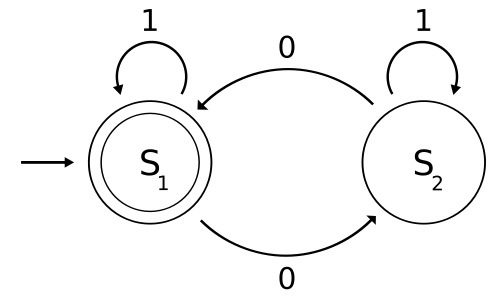
\includegraphics[width=0.5\textwidth]{Images/state-diagram}
       \caption{Simple state diagram}
       \label{fig:sdiag}
\end{figure}

 \subsection{Quisque ut nisi}
 Pellentesque egestas, neque sit amet convallis pulvinar, justo nulla eleifend augue, ac auctor orci leo non est. Quisque id mi. Ut tincidunt tincidunt erat. Etiam feugiat lorem non metus. Vestibulum dapibus nunc ac augue. Curabitur vestibulum aliquam leo. Praesent egestas neque eu enim. In hac habitasse platea dictumst. Fusce a quam. Etiam ut purus mattis mauris sodales aliquam. Curabitur nisi. Quisque malesuada placerat nisl. Nam ipsum risus, rutrum vitae, vestibulum eu, molestie vel, lacus. Sed augue ipsum, egestas nec, vestibulum et, malesuada adipiscing, dui. Vestibulum facilisis, purus nec pulvinar iaculis, ligula mi congue nunc, vitae euismod ligula urna in dolor. Mauris sollicitudin fermentum libero. Praesent nonummy mi in odio. Nunc interdum lacus sit amet orci. Vestibulum rutrum, mi nec elementum vehicula, eros quam gravida nisl, id fringilla neque ante vel mi. Morbi mollis tellus ac sapien. Phasellus volutpat, metus eget egestas mollis, lacus lacus blandit dui, id egestas quam mauris ut lacus. Fusce vel dui. Sed in libero ut nibh placerat accumsan. Proin faucibus arcu quis ante. In consectetuer turpis ut velit. Nulla sit amet est. Praesent metus tellus, elementum eu, semper a, adipiscing nec, purus. Cras risus ipsum, faucibus ut, ullamcorper id, varius ac, leo. Suspendisse feugiat. Suspendisse enim turpis, dictum sed, iaculis a, condimentum nec, nisi. Praesent nec nisl a purus blandit viverra. Praesent ac massa at ligula laoreet iaculis. Nulla neque dolor, sagittis eget, iaculis quis, molestie non, velit. Mauris turpis nunc, blandit et, volutpat molestie, porta ut, ligula. Fusce pharetra convallis urna. Quisque ut nisi. Donec mi odio, faucibus at, scelerisque quis, convallis in, nisi.

 \subsection{Nam adipiscing}
 Suspendisse non nisl sit amet velit hendrerit rutrum. Ut leo. Ut a nisl id ante tempus hendrerit. Proin pretium, leo ac pellentesque mollis, felis nunc ultrices eros, sed gravida augue augue mollis justo. Suspendisse eu ligula. Nulla facilisi. Donec id justo. Praesent porttitor, nulla vitae posuere iaculis, arcu nisl dignissim dolor, a pretium mi sem ut ipsum. Curabitur suscipit suscipit tellus. Praesent vestibulum dapibus nibh. Etiam iaculis nunc ac metus. Ut id nisl quis enim dignissim sagittis. Etiam sollicitudin, ipsum eu pulvinar rutrum, tellus ipsum laoreet sapien, quis venenatis ante odio sit amet eros. Proin magna. Duis vel nibh at velit scelerisque suscipit. Curabitur turpis. Vestibulum suscipit nulla quis orci. Fusce ac felis sit amet ligula pharetra condimentum. Maecenas egestas arcu quis ligula mattis placerat. Duis lobortis massa imperdiet quam. Suspendisse potenti. Pellentesque commodo eros a enim. Vestibulum turpis sem, aliquet eget, lobortis pellentesque, rutrum eu, nisl. Sed libero. Aliquam erat volutpat. Etiam vitae tortor. Morbi vestibulum volutpat enim. Aliquam eu nunc. Nunc sed turpis. Sed mollis, eros et ultrices tempus, mauris ipsum aliquam libero, non adipiscing dolor urna a orci. Nulla porta dolor. Class aptent taciti sociosqu ad litora torquent per conubia nostra, per inceptos hymenaeos. Pellentesque dapibus hendrerit tortor. Praesent egestas tristique nibh. Sed a libero. Cras varius. Donec vitae orci sed dolor rutrum auctor. Fusce egestas elit eget lorem. Suspendisse nisl elit, rhoncus eget, elementum ac, condimentum eget, diam. Nam at tortor in tellus interdum sagittis. Aliquam lobortis. Donec orci lectus, aliquam ut, faucibus non, euismod id, nulla. Curabitur blandit mollis lacus. Nam adipiscing.

 Vestibulum eu odio. Vivamus laoreet. Nullam tincidunt adipiscing enim. Phasellus tempus. Proin viverra, ligula sit amet ultrices semper, ligula arcu tristique sapien, a accumsan nisi mauris ac eros. Fusce neque. Suspendisse faucibus, nunc et pellentesque egestas, lacus ante convallis tellus, vitae iaculis lacus elit id tortor. Vivamus aliquet elit ac nisl. Fusce fermentum odio nec arcu. Vivamus euismod mauris. In ut quam vitae odio lacinia tincidunt. Praesent ut ligula non mi varius sagittis. Cras sagittis. Praesent ac sem eget est egestas volutpat. Vivamus consectetuer hendrerit lacus. Cras non dolor. Vivamus in erat ut urna cursus vestibulum. Fusce commodo aliquam arcu. Nam commodo suscipit quam. Quisque id odio. Praesent venenatis metus at tortor pulvinar varius. Lorem ipsum dolor sit amet, consectetuer adipiscing elit. Aenean commodo ligula eget dolor. Aenean massa. Cum sociis natoque penatibus et magnis dis parturient montes, nascetur ridiculus mus. Donec quam felis, ultricies nec, pellentesque eu, pretium quis, sem. Nulla consequat massa quis enim. Donec pede justo, fringilla vel, aliquet nec, vulputate eget, arcu. In enim justo, rhoncus ut, imperdiet a, venenatis vitae, justo. Nullam dictum felis eu pede mollis pretium. Integer tincidunt. Cras dapibus. Vivamus elementum semper nisi. Aenean vulputate eleifend tellus. Aenean leo ligula, porttitor eu, consequat vitae, eleifend ac, enim. Aliquam lorem ante, dapibus in, viverra quis, feugiat a, tellus. Phasellus viverra nulla ut metus varius laoreet. Quisque rutrum. Aenean imperdiet. Etiam ultricies nisi vel augue. Curabitur ullamcorper ultricies nisi. Nam eget dui. Etiam rhoncus.

 \section{Donec id justo}
 Maecenas tempus, tellus eget condimentum rhoncus, sem quam semper libero, sit amet adipiscing sem neque sed ipsum. Nam quam nunc, blandit vel, luctus pulvinar, hendrerit id, lorem. Maecenas nec odio et ante tincidunt tempus. Donec vitae sapien ut libero venenatis faucibus. Nullam quis ante. Etiam sit amet orci eget eros faucibus tincidunt. Duis leo. Sed fringilla mauris sit amet nibh. Donec sodales sagittis magna. Sed consequat, leo eget bibendum sodales, augue velit cursus nunc, quis gravida magna mi a libero. Fusce vulputate eleifend sapien. Vestibulum purus quam, scelerisque ut, mollis sed, nonummy id, metus. Nullam accumsan lorem in dui. Cras ultricies mi eu turpis hendrerit fringilla. Vestibulum ante ipsum primis in faucibus orci luctus et ultrices posuere cubilia Curae; In ac dui quis mi consectetuer lacinia. Nam pretium turpis et arcu. Duis arcu tortor, suscipit eget, imperdiet nec, imperdiet iaculis, ipsum. Sed aliquam ultrices mauris. Integer ante arcu, accumsan a, consectetuer eget, posuere ut, mauris. Praesent adipiscing. Phasellus ullamcorper ipsum rutrum nunc. Nunc nonummy metus. Vestibulum volutpat pretium libero. Cras id dui. Aenean ut eros et nisl sagittis vestibulum. Nullam nulla eros, ultricies sit amet, nonummy id, imperdiet feugiat, pede. Sed lectus. Donec mollis hendrerit risus. Phasellus nec sem in justo pellentesque facilisis. Etiam imperdiet imperdiet orci. Nunc nec neque. Phasellus leo dolor, tempus non, auctor et, hendrerit quis, nisi. Curabitur ligula sapien, tincidunt non, euismod vitae, posuere imperdiet, leo. Maecenas malesuada. Praesent congue erat at massa. Sed cursus turpis vitae tortor. Donec posuere vulputate arcu. Phasellus accumsan cursus velit.

 Vestibulum ante ipsum primis in faucibus orci luctus et ultrices posuere cubilia Curae; Sed aliquam, nisi quis porttitor congue, elit erat euismod orci, ac placerat dolor lectus quis orci. Phasellus consectetuer vestibulum elit. Aenean tellus metus, bibendum sed, posuere ac, mattis non, nunc. Vestibulum fringilla pede sit amet augue. In turpis. Pellentesque posuere. Praesent turpis. Aenean posuere, tortor sed cursus feugiat, nunc augue blandit nunc, eu sollicitudin urna dolor sagittis lacus. Donec elit libero, sodales nec, volutpat a, suscipit non, turpis. Nullam sagittis. Suspendisse pulvinar, augue ac venenatis condimentum, sem libero volutpat nibh, nec pellentesque velit pede quis nunc. Vestibulum ante ipsum primis in faucibus orci luctus et ultrices posuere cubilia Curae; Fusce id purus. Ut varius tincidunt libero. Phasellus dolor. Maecenas vestibulum mollis diam. Pellentesque ut neque. Pellentesque habitant morbi tristique senectus et netus et malesuada fames ac turpis egestas. In dui magna, posuere eget, vestibulum et, tempor auctor, justo. In ac felis quis tortor malesuada pretium. Pellentesque auctor neque nec urna. Proin sapien ipsum, porta a, auctor quis, euismod ut, mi. Aenean viverra rhoncus pede. Pellentesque habitant morbi tristique senectus et netus et malesuada fames ac turpis egestas. Ut non enim eleifend felis pretium feugiat. Vivamus quis mi. Phasellus a est. Phasellus magna. In hac habitasse platea dictumst. Curabitur at lacus ac velit ornare lobortis. Curabitur a felis in nunc fringilla tristique. Morbi mattis ullamcorper velit. Phasellus gravida semper nisi. Nullam vel sem. Pellentesque libero tortor, tincidunt et, tincidunt eget, semper nec, quam. Sed hendrerit. Morbi ac felis.
 
  \begin{center}
     \begin{tabular}{ | l | l | l | p{7cm} |}
     \hline
     Day & Min Temp & Max Temp & Summary \\ \hline
     Monday & 11C & 22C & A clear day with lots of sunshine.  
     However, the strong breeze will bring down the temperatures. \\ \hline
     Tuesday & 9C & 19C & Cloudy with rain, across many northern regions. Clear spells
     across most of Scotland and Northern Ireland,
     but rain reaching the far northwest. \\ \hline
     Wednesday & 10C & 21C & Rain will still linger for the morning.
     Conditions will improve by early afternoon and continue
     throughout the evening. \\
     \hline
     \end{tabular}
\end{center}

%==================================================
%Second enumerated chapter
%==================================================
\chapter{Sed augue}
\lettrine[nindent=0em,lines=3]{M} aecenas tempus, tellus eget condimentum rhoncus, sem quam semper libero, sit amet adipiscing sem neque sed ipsum. Nam quam nunc, blandit vel, luctus pulvinar, hendrerit id, lorem. Maecenas nec odio et ante tincidunt tempus. Donec vitae sapien ut libero venenatis faucibus. Nullam quis ante. Etiam sit amet orci eget eros faucibus tincidunt. Duis leo. Sed fringilla mauris sit amet nibh. Donec sodales sagittis magna. Sed consequat, leo eget bibendum sodales, augue velit cursus nunc, quis gravida magna mi a libero. Fusce vulputate eleifend sapien. Vestibulum purus quam, scelerisque ut, mollis sed, nonummy id, metus. Nullam accumsan lorem in dui. Cras ultricies mi eu turpis hendrerit fringilla. Vestibulum ante ipsum primis in faucibus orci luctus et ultrices posuere cubilia Curae; In ac dui quis mi consectetuer lacinia. Nam pretium turpis et arcu. Duis arcu tortor, suscipit eget, imperdiet nec, imperdiet iaculis, ipsum. Sed aliquam ultrices mauris. Integer ante arcu, accumsan a, consectetuer eget, posuere ut, mauris. Praesent adipiscing. Phasellus ullamcorper ipsum rutrum nunc. Nunc nonummy metus. Vestibulum volutpat pretium libero. Cras id dui. Aenean ut eros et nisl sagittis vestibulum. Nullam nulla eros, ultricies sit amet, nonummy id, imperdiet feugiat, pede. Sed lectus. Donec mollis hendrerit risus. Phasellus nec sem in justo pellentesque facilisis. Etiam imperdiet imperdiet orci. Nunc nec neque. Phasellus leo dolor, tempus non, auctor et, hendrerit quis, nisi. Curabitur ligula sapien, tincidunt non, euismod vitae, posuere imperdiet, leo. Maecenas malesuada. Praesent congue erat at massa. Sed cursus turpis vitae tortor. Donec posuere vulputate arcu. Phasellus accumsan cursus velit.

\section{Phasellus leo dolor}
Vestibulum ante ipsum primis in faucibus orci luctus et ultrices posuere cubilia Curae; Sed aliquam, nisi quis porttitor congue, elit erat euismod orci, ac placerat dolor lectus quis orci. Phasellus consectetuer vestibulum elit. Aenean tellus metus, bibendum sed, posuere ac, mattis non, nunc. Vestibulum fringilla pede sit amet augue. In turpis. Pellentesque posuere. Praesent turpis. Aenean posuere, tortor sed cursus feugiat, nunc augue blandit nunc, eu sollicitudin urna dolor sagittis lacus. Donec elit libero, sodales nec, volutpat a, suscipit non, turpis. Nullam sagittis. Suspendisse pulvinar, augue ac venenatis condimentum, sem libero volutpat nibh, nec pellentesque velit pede quis nunc. Vestibulum ante ipsum primis in faucibus orci luctus et ultrices posuere cubilia Curae; Fusce id purus. Ut varius tincidunt libero. Phasellus dolor. Maecenas vestibulum mollis diam. Pellentesque ut neque. Pellentesque habitant morbi tristique senectus et netus et malesuada fames ac turpis egestas. In dui magna, posuere eget, vestibulum et, tempor auctor, justo. In ac felis quis tortor malesuada pretium. Pellentesque auctor neque nec urna. Proin sapien ipsum, porta a, auctor quis, euismod ut, mi. Aenean viverra rhoncus pede. Pellentesque habitant morbi tristique senectus et netus et malesuada fames ac turpis egestas. Ut non enim eleifend felis pretium feugiat. Vivamus quis mi. Phasellus a est. Phasellus magna. In hac habitasse platea dictumst. Curabitur at lacus ac velit ornare lobortis. Curabitur a felis in nunc fringilla tristique. Morbi mattis ullamcorper velit. Phasellus gravida semper nisi. Nullam vel sem. Pellentesque libero tortor, tincidunt et, tincidunt eget, semper nec, quam. Sed hendrerit. Morbi ac felis.

Nunc egestas, augue at pellentesque laoreet, felis eros vehicula leo, at malesuada velit leo quis pede. Donec interdum, metus et hendrerit aliquet, dolor diam sagittis ligula, eget egestas libero turpis vel mi. Nunc nulla. Fusce risus nisl, viverra et, tempor et, pretium in, sapien. Donec venenatis vulputate lorem. Morbi nec metus. Phasellus blandit leo ut odio. Maecenas ullamcorper, dui et placerat feugiat, eros pede varius nisi, condimentum viverra felis nunc et lorem. Sed magna purus, fermentum eu, tincidunt eu, varius ut, felis. In auctor lobortis lacus. Quisque libero metus, condimentum nec, tempor a, commodo mollis, magna. Vestibulum ullamcorper mauris at ligula. Fusce fermentum. Nullam cursus lacinia erat. Praesent blandit laoreet nibh. Fusce convallis metus id felis luctus adipiscing. Pellentesque egestas, neque sit amet convallis pulvinar, justo nulla eleifend augue, ac auctor orci leo non est. Quisque id mi. Ut tincidunt tincidunt erat. Etiam feugiat lorem non metus. Vestibulum dapibus nunc ac augue. Curabitur vestibulum aliquam leo. Praesent egestas neque eu enim. In hac habitasse platea dictumst. Fusce a quam. Etiam ut purus mattis mauris sodales aliquam. Curabitur nisi. Quisque malesuada placerat nisl. Nam ipsum risus, rutrum vitae, vestibulum eu, molestie vel, lacus. Sed augue ipsum, egestas nec, vestibulum et, malesuada adipiscing, dui. Vestibulum facilisis, purus nec pulvinar iaculis, ligula mi congue nunc, vitae euismod ligula urna in dolor. Mauris sollicitudin fermentum libero. Praesent nonummy mi in odio. Nunc interdum lacus sit amet orci. Vestibulum rutrum, mi nec elementum vehicula, eros quam gravida nisl, id fringilla neque ante vel mi. Morbi mollis tellus ac sapien.

\section{Nullam vel sem}
Phasellus volutpat, metus eget egestas mollis, lacus lacus blandit dui, id egestas quam mauris ut lacus. Fusce vel dui. Sed in libero ut nibh placerat accumsan. Proin faucibus arcu quis ante. In consectetuer turpis ut velit. Nulla sit amet est. Praesent metus tellus, elementum eu, semper a, adipiscing nec, purus. Cras risus ipsum, faucibus ut, ullamcorper id, varius ac, leo. Suspendisse feugiat. Suspendisse enim turpis, dictum sed, iaculis a, condimentum nec, nisi. Praesent nec nisl a purus blandit viverra. Praesent ac massa at ligula laoreet iaculis. Nulla neque dolor, sagittis eget, iaculis quis, molestie non, velit. Mauris turpis nunc, blandit et, volutpat molestie, porta ut, ligula. Fusce pharetra convallis urna. Quisque ut nisi. Donec mi odio, faucibus at, scelerisque quis, convallis in, nisi. Suspendisse non nisl sit amet velit hendrerit rutrum. Ut leo. Ut a nisl id ante tempus hendrerit. Proin pretium, leo ac pellentesque mollis, felis nunc ultrices eros, sed gravida augue augue mollis justo. Suspendisse eu ligula. Nulla facilisi. Donec id justo. Praesent porttitor, nulla vitae posuere iaculis, arcu nisl dignissim dolor, a pretium mi sem ut ipsum. Curabitur suscipit suscipit tellus. Praesent vestibulum dapibus nibh. Etiam iaculis nunc ac metus. Ut id nisl quis enim dignissim sagittis. Etiam sollicitudin, ipsum eu pulvinar rutrum, tellus ipsum laoreet sapien, quis venenatis ante odio sit amet eros. Proin magna. Duis vel nibh at velit scelerisque suscipit. Curabitur turpis. Vestibulum suscipit nulla quis orci. Fusce ac felis sit amet ligula pharetra condimentum. Maecenas egestas arcu quis ligula mattis placerat. Duis lobortis massa imperdiet quam. Suspendisse potenti. Pellentesque commodo eros a enim.

Vestibulum turpis sem, aliquet eget, lobortis pellentesque, rutrum eu, nisl. Sed libero. Aliquam erat volutpat. Etiam vitae tortor. Morbi vestibulum volutpat enim. Aliquam eu nunc. Nunc sed turpis. Sed mollis, eros et ultrices tempus, mauris ipsum aliquam libero, non adipiscing dolor urna a orci. Nulla porta dolor. Class aptent taciti sociosqu ad litora torquent per conubia nostra, per inceptos hymenaeos. Pellentesque dapibus hendrerit tortor. Praesent egestas tristique nibh. Sed a libero. Cras varius. Donec vitae orci sed dolor rutrum auctor. Fusce egestas elit eget lorem. Suspendisse nisl elit, rhoncus eget, elementum ac, condimentum eget, diam. Nam at tortor in tellus interdum sagittis. Aliquam lobortis. Donec orci lectus, aliquam ut, faucibus non, euismod id, nulla. Curabitur blandit mollis lacus. Nam adipiscing. Vestibulum eu odio. Vivamus laoreet. Nullam tincidunt adipiscing enim. Phasellus tempus. Proin viverra, ligula sit amet ultrices semper, ligula arcu tristique sapien, a accumsan nisi mauris ac eros. Fusce neque. Suspendisse faucibus, nunc et pellentesque egestas, lacus ante convallis tellus, vitae iaculis lacus elit id tortor. Vivamus aliquet elit ac nisl. Fusce fermentum odio nec arcu. Vivamus euismod mauris. In ut quam vitae odio lacinia tincidunt. Praesent ut ligula non mi varius sagittis. Cras sagittis. Praesent ac sem eget est egestas volutpat. Vivamus consectetuer hendrerit lacus. Cras non dolor. Vivamus in erat ut urna cursus vestibulum. Fusce commodo aliquam arcu. Nam commodo suscipit quam. Quisque id odio. Praesent venenatis metus at tortor pulvinar varius. Lorem ipsum dolor sit amet, consectetuer adipiscing elit. Aenean commodo ligula eget dolor. Aenean massa. Cum sociis natoque penatibus et magnis dis parturient montes, nascetur ridiculus mus.

\section{Morbi mollis tellus}
Donec quam felis, ultricies nec, pellentesque eu, pretium quis, sem. Nulla consequat massa quis enim. Donec pede justo, fringilla vel, aliquet nec, vulputate eget, arcu. In enim justo, rhoncus ut, imperdiet a, venenatis vitae, justo. Nullam dictum felis eu pede mollis pretium. Integer tincidunt. Cras dapibus. Vivamus elementum semper nisi. Aenean vulputate eleifend tellus. Aenean leo ligula, porttitor eu, consequat vitae, eleifend ac, enim. Aliquam lorem ante, dapibus in, viverra quis, feugiat a, tellus. Phasellus viverra nulla ut metus varius laoreet. Quisque rutrum. Aenean imperdiet. Etiam ultricies nisi vel augue. Curabitur ullamcorper ultricies nisi. Nam eget dui. Etiam rhoncus. Maecenas tempus, tellus eget condimentum rhoncus, sem quam semper libero, sit amet adipiscing sem neque sed ipsum. Nam quam nunc, blandit vel, luctus pulvinar, hendrerit id, lorem. Maecenas nec odio et ante tincidunt tempus. Donec vitae sapien ut libero venenatis faucibus. Nullam quis ante. Etiam sit amet orci eget eros faucibus tincidunt. Duis leo. Sed fringilla mauris sit amet nibh. Donec sodales sagittis magna. Sed consequat, leo eget bibendum sodales, augue velit cursus nunc, quis gravida magna mi a libero. Fusce vulputate eleifend sapien. Vestibulum purus quam, scelerisque ut, mollis sed, nonummy id, metus. Nullam accumsan lorem in dui. Cras ultricies mi eu turpis hendrerit fringilla. Vestibulum ante ipsum primis in faucibus orci luctus et ultrices posuere cubilia Curae; In ac dui quis mi consectetuer lacinia. Nam pretium turpis et arcu. Duis arcu tortor, suscipit eget, imperdiet nec, imperdiet iaculis, ipsum. Sed aliquam ultrices mauris. Integer ante arcu, accumsan a, consectetuer eget, posuere ut, mauris. Praesent adipiscing. Phasellus ullamcorper ipsum rutrum nunc. Nunc nonummy metus.

Vestibulum volutpat pretium libero. Cras id dui. Aenean ut eros et nisl sagittis vestibulum. Nullam nulla eros, ultricies sit amet, nonummy id, imperdiet feugiat, pede. Sed lectus. Donec mollis hendrerit risus. Phasellus nec sem in justo pellentesque facilisis. Etiam imperdiet imperdiet orci. Nunc nec neque. Phasellus leo dolor, tempus non, auctor et, hendrerit quis, nisi. Curabitur ligula sapien, tincidunt non, euismod vitae, posuere imperdiet, leo. Maecenas malesuada. Praesent congue erat at massa. Sed cursus turpis vitae tortor. Donec posuere vulputate arcu. Phasellus accumsan cursus velit. Vestibulum ante ipsum primis in faucibus orci luctus et ultrices posuere cubilia Curae; Sed aliquam, nisi quis porttitor congue, elit erat euismod orci, ac placerat dolor lectus quis orci. Phasellus consectetuer vestibulum elit. Aenean tellus metus, bibendum sed, posuere ac, mattis non, nunc. Vestibulum fringilla pede sit amet augue. In turpis. Pellentesque posuere. Praesent turpis. Aenean posuere, tortor sed cursus feugiat, nunc augue blandit nunc, eu sollicitudin urna dolor sagittis lacus. Donec elit libero, sodales nec, volutpat a, suscipit non, turpis. Nullam sagittis. Suspendisse pulvinar, augue ac venenatis condimentum, sem libero volutpat nibh, nec pellentesque velit pede quis nunc. Vestibulum ante ipsum primis in faucibus orci luctus et ultrices posuere cubilia Curae; Fusce id purus. Ut varius tincidunt libero. Phasellus dolor. Maecenas vestibulum mollis diam. Pellentesque ut neque. Pellentesque habitant morbi tristique senectus et netus et malesuada fames ac turpis egestas. In dui magna, posuere eget, vestibulum et, tempor auctor, justo. In ac felis quis tortor malesuada pretium. Pellentesque auctor neque nec urna. Proin sapien ipsum, porta a, auctor quis, euismod ut, mi.

%==================================================
%Third enumerated chapter
%==================================================
\chapter{Donec sodales sagittis magna}
\lettrine[nindent=0em,lines=3]{N} am ipsum risus, rutrum vitae, vestibulum eu, molestie vel, lacus. Sed augue ipsum, egestas nec, vestibulum et, malesuada adipiscing, dui. Vestibulum facilisis, purus nec pulvinar iaculis, ligula mi congue nunc, vitae euismod ligula urna in dolor. Mauris sollicitudin fermentum libero. Praesent nonummy mi in odio. Nunc interdum lacus sit amet orci. Vestibulum rutrum, mi nec elementum vehicula, eros quam gravida nisl, id fringilla neque ante vel mi. Morbi mollis tellus ac sapien. Phasellus volutpat, metus eget egestas mollis, lacus lacus blandit dui, id egestas quam mauris ut lacus. Fusce vel dui. Sed in libero ut nibh placerat accumsan. Proin faucibus arcu quis ante. In consectetuer turpis ut velit. Nulla sit amet est. Praesent metus tellus, elementum eu, semper a, adipiscing nec, purus. Cras risus ipsum, faucibus ut, ullamcorper id, varius ac, leo. Suspendisse feugiat. Suspendisse enim turpis, dictum sed, iaculis a, condimentum nec, nisi. Praesent nec nisl a purus blandit viverra. Praesent ac massa at ligula laoreet iaculis. Nulla neque dolor, sagittis eget, iaculis quis, molestie non, velit. Mauris turpis nunc, blandit et, volutpat molestie, porta ut, ligula. Fusce pharetra convallis urna. Quisque ut nisi. Donec mi odio, faucibus at, scelerisque quis, convallis in, nisi. Suspendisse non nisl sit amet velit hendrerit rutrum. Ut leo. Ut a nisl id ante tempus hendrerit. Proin pretium, leo ac pellentesque mollis, felis nunc ultrices eros, sed gravida augue augue mollis justo. Suspendisse eu ligula. Nulla facilisi. Donec id justo. Praesent porttitor, nulla vitae posuere iaculis, arcu nisl dignissim dolor, a pretium mi sem ut ipsum. Curabitur suscipit suscipit tellus. Praesent vestibulum dapibus nibh. Etiam iaculis nunc ac metus. Ut id nisl quis enim dignissim sagittis. Etiam sollicitudin, ipsum eu pulvinar rutrum, tellus ipsum laoreet sapien, quis venenatis ante odio sit amet eros. Proin magna. Duis vel nibh at velit scelerisque suscipit. Curabitur turpis. Vestibulum suscipit nulla quis orci. Fusce ac felis sit amet ligula pharetra condimentum. Maecenas egestas arcu quis ligula mattis placerat. Duis lobortis massa imperdiet quam. Suspendisse potenti. Pellentesque commodo eros a enim. Vestibulum turpis sem, aliquet eget, lobortis pellentesque, rutrum eu, nisl. Sed libero. Aliquam erat volutpat. Etiam vitae tortor. Morbi vestibulum volutpat enim. Aliquam eu nunc. Nunc sed turpis. Sed mollis, eros et ultrices tempus, mauris ipsum aliquam libero, non adipiscing dolor urna a orci. Nulla porta dolor. Class aptent taciti sociosqu ad litora torquent per conubia nostra, per inceptos hymenaeos. Pellentesque dapibus hendrerit tortor. Praesent egestas tristique nibh. Sed a libero. Cras varius. Donec vitae orci sed dolor rutrum auctor. Fusce egestas elit eget lorem. Suspendisse nisl elit, rhoncus eget, elementum ac, condimentum eget, diam. Nam at tortor in tellus interdum sagittis. Aliquam lobortis. Donec orci lectus, aliquam ut, faucibus non, euismod

\section{Proin pretium}
\subsection{Aliquam lobortis}
Duis arcu tortor, suscipit eget, imperdiet nec, imperdiet iaculis, ipsum. Sed aliquam ultrices mauris. Integer ante arcu, accumsan a, consectetuer eget, posuere ut, mauris. Praesent adipiscing. Phasellus ullamcorper ipsum rutrum nunc. Nunc nonummy metus. Vestibulum volutpat pretium libero. Cras id dui. Aenean ut eros et nisl sagittis vestibulum. Nullam nulla eros, ultricies sit amet, nonummy id, imperdiet feugiat, pede. Sed lectus. Donec mollis hendrerit risus. Phasellus nec sem in justo pellentesque facilisis. Etiam imperdiet imperdiet orci. Nunc nec neque. Phasellus leo dolor, tempus non, auctor et, hendrerit quis, nisi. Curabitur ligula sapien, tincidunt non, euismod vitae, posuere imperdiet, leo. Maecenas malesuada. Praesent congue erat at massa. Sed cursus turpis vitae tortor. Donec posuere vulputate arcu. Phasellus accumsan cursus velit. Vestibulum ante ipsum primis in faucibus orci luctus et ultrices posuere cubilia Curae; Sed aliquam, nisi quis porttitor congue, elit erat euismod orci, ac placerat dolor lectus quis orci. Phasellus consectetuer vestibulum elit. Aenean tellus metus, bibendum sed, posuere ac, mattis non, nunc. Vestibulum fringilla pede sit amet augue. In turpis. Pellentesque posuere. Praesent turpis. Aenean posuere, tortor sed cursus feugiat, nunc augue blandit nunc, eu sollicitudin urna dolor sagittis lacus. Donec elit libero, sodales nec, volutpat a, suscipit non, turpis. Nullam sagittis. Suspendisse pulvinar, augue ac venenatis condimentum, sem libero volutpat nibh, nec pellentesque velit pede quis nunc. Vestibulum ante ipsum primis in faucibus orci luctus et ultrices posuere cubilia Curae; Fusce id purus. Ut varius tincidunt libero. Phasellus dolor. Maecenas vestibulum mollis diam.

Pellentesque ut neque. Pellentesque habitant morbi tristique senectus et netus et malesuada fames ac turpis egestas. In dui magna, posuere eget, vestibulum et, tempor auctor, justo. In ac felis quis tortor malesuada pretium. Pellentesque auctor neque nec urna. Proin sapien ipsum, porta a, auctor quis, euismod ut, mi. Aenean viverra rhoncus pede. Pellentesque habitant morbi tristique senectus et netus et malesuada fames ac turpis egestas. Ut non enim eleifend felis pretium feugiat. Vivamus quis mi. Phasellus a est. Phasellus magna. In hac habitasse platea dictumst. Curabitur at lacus ac velit ornare lobortis. Curabitur a felis in nunc fringilla tristique. Morbi mattis ullamcorper velit. Phasellus gravida semper nisi. Nullam vel sem. Pellentesque libero tortor, tincidunt et, tincidunt eget, semper nec, quam. Sed hendrerit. Morbi ac felis. Nunc egestas, augue at pellentesque laoreet, felis eros vehicula leo, at malesuada velit leo quis pede. Donec interdum, metus et hendrerit aliquet, dolor diam sagittis ligula, eget egestas libero turpis vel mi. Nunc nulla. Fusce risus nisl, viverra et, tempor et, pretium in, sapien. Donec venenatis vulputate lorem. Morbi nec metus. Phasellus blandit leo ut odio. Maecenas ullamcorper, dui et placerat feugiat, eros pede varius nisi, condimentum viverra felis nunc et lorem. Sed magna purus, fermentum eu, tincidunt eu, varius ut, felis. In auctor lobortis lacus. Quisque libero metus, condimentum nec, tempor a, commodo mollis, magna. Vestibulum ullamcorper mauris at ligula. Fusce fermentum. Nullam cursus lacinia erat. Praesent blandit laoreet nibh. Fusce convallis metus id felis luctus adipiscing.

\subsection{Curabitur blandit mollis lacus}
Pellentesque egestas, neque sit amet convallis pulvinar, justo nulla eleifend augue, ac auctor orci leo non est. Quisque id mi. Ut tincidunt tincidunt erat. Etiam feugiat lorem non metus. Vestibulum dapibus nunc ac augue. Curabitur vestibulum aliquam leo. Praesent egestas neque eu enim. In hac habitasse platea dictumst. Fusce a quam. Etiam ut purus mattis mauris sodales aliquam. Curabitur nisi. Quisque malesuada placerat nisl. Nam ipsum risus, rutrum vitae, vestibulum eu, molestie vel, lacus. Sed augue ipsum, egestas nec, vestibulum et, malesuada adipiscing, dui. Vestibulum facilisis, purus nec pulvinar iaculis, ligula mi congue nunc, vitae euismod ligula urna in dolor. Mauris sollicitudin fermentum libero. Praesent nonummy mi in odio. Nunc interdum lacus sit amet orci. Vestibulum rutrum, mi nec elementum vehicula, eros quam gravida nisl, id fringilla neque ante vel mi. Morbi mollis tellus ac sapien. Phasellus volutpat, metus eget egestas mollis, lacus lacus blandit dui, id egestas quam mauris ut lacus. Fusce vel dui. Sed in libero ut nibh placerat accumsan. Proin faucibus arcu quis ante. In consectetuer turpis ut velit. Nulla sit amet est. Praesent metus tellus, elementum eu, semper a, adipiscing nec, purus. Cras risus ipsum, faucibus ut, ullamcorper id, varius ac, leo. Suspendisse feugiat. Suspendisse enim turpis, dictum sed, iaculis a, condimentum nec, nisi. Praesent nec nisl a purus blandit viverra. Praesent ac massa at ligula laoreet iaculis. Nulla neque dolor, sagittis eget, iaculis quis, molestie non, velit. Mauris turpis nunc, blandit et, volutpat molestie, porta ut, ligula. Fusce pharetra convallis urna. Quisque ut nisi. Donec mi odio, faucibus at, scelerisque quis, convallis in, nisi.

Suspendisse non nisl sit amet velit hendrerit rutrum. Ut leo. Ut a nisl id ante tempus hendrerit. Proin pretium, leo ac pellentesque mollis, felis nunc ultrices eros, sed gravida augue augue mollis justo. Suspendisse eu ligula. Nulla facilisi. Donec id justo. Praesent porttitor, nulla vitae posuere iaculis, arcu nisl dignissim dolor, a pretium mi sem ut ipsum. Curabitur suscipit suscipit tellus. Praesent vestibulum dapibus nibh. Etiam iaculis nunc ac metus. Ut id nisl quis enim dignissim sagittis. Etiam sollicitudin, ipsum eu pulvinar rutrum, tellus ipsum laoreet sapien, quis venenatis ante odio sit amet eros. Proin magna. Duis vel nibh at velit scelerisque suscipit. Curabitur turpis. Vestibulum suscipit nulla quis orci. Fusce ac felis sit amet ligula pharetra condimentum. Maecenas egestas arcu quis ligula mattis placerat. Duis lobortis massa imperdiet quam. Suspendisse potenti. Pellentesque commodo eros a enim. Vestibulum turpis sem, aliquet eget, lobortis pellentesque, rutrum eu, nisl. Sed libero. Aliquam erat volutpat. Etiam vitae tortor. Morbi vestibulum volutpat enim. Aliquam eu nunc. Nunc sed turpis. Sed mollis, eros et ultrices tempus, mauris ipsum aliquam libero, non adipiscing dolor urna a orci. Nulla porta dolor. Class aptent taciti sociosqu ad litora torquent per conubia nostra, per inceptos hymenaeos. Pellentesque dapibus hendrerit tortor. Praesent egestas tristique nibh. Sed a libero. Cras varius. Donec vitae orci sed dolor rutrum auctor. Fusce egestas elit eget lorem. Suspendisse nisl elit, rhoncus eget, elementum ac, condimentum eget, diam. Nam at tortor in tellus interdum sagittis. Aliquam lobortis. Donec orci lectus, aliquam ut, faucibus non, euismod id, nulla. Curabitur blandit mollis lacus. Nam adipiscing.

\section{Duis leo}
Vestibulum eu odio. Vivamus laoreet. Nullam tincidunt adipiscing enim. Phasellus tempus. Proin viverra, ligula sit amet ultrices semper, ligula arcu tristique sapien, a accumsan nisi mauris ac eros. Fusce neque. Suspendisse faucibus, nunc et pellentesque egestas, lacus ante convallis tellus, vitae iaculis lacus elit id tortor. Vivamus aliquet elit ac nisl. Fusce fermentum odio nec arcu. Vivamus euismod mauris. In ut quam vitae odio lacinia tincidunt. Praesent ut ligula non mi varius sagittis. Cras sagittis. Praesent ac sem eget est egestas volutpat. Vivamus consectetuer hendrerit lacus. Cras non dolor. Vivamus in erat ut urna cursus vestibulum. Fusce commodo aliquam arcu. Nam commodo suscipit quam. Quisque id odio. Praesent venenatis metus at tortor pulvinar varius. Lorem ipsum dolor sit amet, consectetuer adipiscing elit. Aenean commodo ligula eget dolor. Aenean massa. Cum sociis natoque penatibus et magnis dis parturient montes, nascetur ridiculus mus. Donec quam felis, ultricies nec, pellentesque eu, pretium quis, sem. Nulla consequat massa quis enim. Donec pede justo, fringilla vel, aliquet nec, vulputate eget, arcu. In enim justo, rhoncus ut, imperdiet a, venenatis vitae, justo. Nullam dictum felis eu pede mollis pretium. Integer tincidunt. Cras dapibus. Vivamus elementum semper nisi. Aenean vulputate eleifend tellus. Aenean leo ligula, porttitor eu, consequat vitae, eleifend ac, enim. Aliquam lorem ante, dapibus in, viverra quis, feugiat a, tellus. Phasellus viverra nulla ut metus varius laoreet. Quisque rutrum. Aenean imperdiet. Etiam ultricies nisi vel augue. Curabitur ullamcorper ultricies nisi. Nam eget dui. Etiam rhoncus.

Nunc egestas, augue at pellentesque laoreet, felis eros vehicula leo, at malesuada velit leo quis pede. Donec interdum, metus et hendrerit aliquet, dolor diam sagittis ligula, eget egestas libero turpis vel mi. Nunc nulla. Fusce risus nisl, viverra et, tempor et, pretium in, sapien. Donec venenatis vulputate lorem. Morbi nec metus. Phasellus blandit leo ut odio. Maecenas ullamcorper, dui et placerat feugiat, eros pede varius nisi, condimentum viverra felis nunc et lorem. Sed magna purus, fermentum eu, tincidunt eu, varius ut, felis. In auctor lobortis lacus. Quisque libero metus, condimentum nec, tempor a, commodo mollis, magna. Vestibulum ullamcorper mauris at ligula. Fusce fermentum. Nullam cursus lacinia erat. Praesent blandit laoreet nibh. Fusce convallis metus id felis luctus adipiscing. Pellentesque egestas, neque sit amet convallis pulvinar, justo nulla eleifend augue, ac auctor orci leo non est. Quisque id mi. Ut tincidunt tincidunt erat. Etiam feugiat lorem non metus. Vestibulum dapibus nunc ac augue. Curabitur vestibulum aliquam leo. Praesent egestas neque eu enim. In hac habitasse platea dictumst. Fusce a quam. Etiam ut purus mattis mauris sodales aliquam. Curabitur nisi. Quisque malesuada placerat nisl. Nam ipsum risus, rutrum vitae, vestibulum eu, molestie vel, lacus. Sed augue ipsum, egestas nec, vestibulum et, malesuada adipiscing, dui. Vestibulum facilisis, purus nec pulvinar iaculis, ligula mi congue nunc, vitae euismod ligula urna in dolor. Mauris sollicitudin fermentum libero. Praesent nonummy mi in odio. Nunc interdum lacus sit amet orci. Vestibulum rutrum, mi nec elementum vehicula, eros quam gravida nisl, id fringilla neque ante vel mi. Morbi mollis tellus ac sapien.

%==================================================
%Bibliography
%==================================================
\nocite{*}
\bibliographystyle{plain}
\bibliography{bibliography}

%Remove page numbers from Bibliography
\pagenumbering{gobble}


\end{document}
